\subsection{DiauproPlugin}

Die DiauproPlugin ist das Plugin, das in der DAW-Anwendung läuft. Es schickt Audiodaten von der DAW-Anwendung durch drei verketteten Prozessoren. Der erste Prozessor ist ein "Null-Prozess Block", die keine tatsächlichen Audio-Verarbeitung berechnet, aber ist für die Erfassung von Daten in Bezug auf Timing nützlich. Der zweite Prozessor ist die VCO-Block, einen Ton auf der Basis empfangen MIDI-Daten generiert. Der dritte Block ist der VCA, der die Amplitude des Tons über die Zeit gestaltet.

\begin{figure}[H]
    \centering
    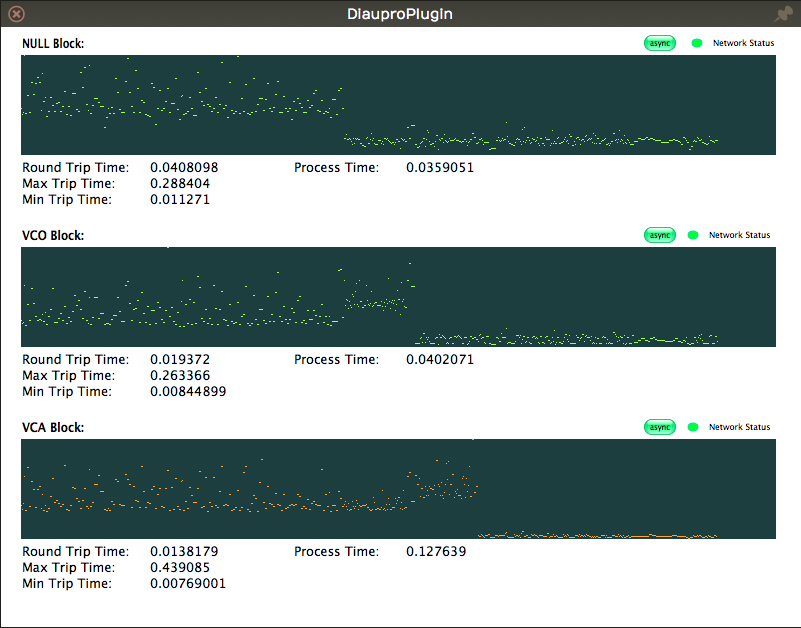
\includegraphics[width=\textwidth]{assets/plugin.png}
    \caption{Screenshot of Plugin GUI}
    \label{fig:plugin}
\end{figure}

Der Benutzeroberfläche des Audio Plugins liefert wichtig informationen in Bezug auf die Zeit und den Status der internen Prozessoren. Jeder Prozessor lokal die Berechnungen lokal auf der CPU ausführen oder zu einem vernetzten Rechenknoten seine Daten senden, um verarbeitet zu werden. Ein "Network Status" Anzeige zeigt, wenn ein Rechenknoten der Verarbeitung übernimmt. Die Gesamtzeit, die ein Prozessor benötigt, um die Operationen durchzuführen wird als "Round Trip Time" angezeigt. "Process Time" ist die Zeit, die eine vernetzte SBC benötigt, um die Verarbeitung durchzuführen.

Ein "async" Knopf ermöglicht dem Benutzer, auf einen asynchronen Verarbeitungsverfahren zu wechseln. Wenn diese aktiviert ist prüft der Prozessor ob Daten von der SBC vorhanden sind, wenn nicht dann wartet es nicht. Stattdessen gibt der Prozessor  einfach leer Daten zurück an den Plugin. Bis der nächste Puffer von der DAW-Anwendung angefordert wird, stehen die ersten Resultate zur Verfügung, und der Prozessor kann diese sofort zurückgeben, ohne zu warten. Diese Methode erzeugt eine Verzögerung in dem Signal von einen Pufferzyklus, hat aber den Vorteil, das es die CPU nicht blockiert. Die Verzögerung kann in der Regel von der DAW-Anwendung kompensiert werden.

Zusätzlich zur Bereitstellung einer grafischen Benutzeroberfläche speichert das Plugin auch Daten in eine Textdatei.